    %==============================================================================
% Voorbeeld gebruik documentklasse hogent-article
%==============================================================================
%
% Compileren in TeXstudio:
%
% - Zorg dat Biber de bibliografie compileert (en niet Biblatex)
%   Options > Configure > Build > Default Bibliography Tool: "txs:///biber"
% - F5 om te compileren en het resultaat te bekijken.
% - Als de bibliografie niet zichtbaar is, probeer dan F5 - F8 - F5
%   Met F8 compileer je de bibliografie apart.
%
% Als je JabRef gebruikt voor het bijhouden van de bibliografie, zorg dan
% dat je in ``biblatex''-modus opslaat: File > Switch to BibLaTeX mode.

\documentclass{hogent-article}

%------------------------------------------------------------------------------
%Custom Commando's
%------------------------------------------------------------------------------
\newcommand{\boldit}[1]{\emph{\textbf{#1}}} 
\newcommand{\customref}[1]{\underline{\ref{#1}: \nameref{#1}}}


%------------------------------------------------------------------------------
% Imports
%------------------------------------------------------------------------------

\graphicspath{{./grafieken/}}
\usepackage{subcaption}
\usepackage{float}
\usepackage{lipsum} % Voor vultekst


%---------- Titel & auteur ----------------------------------------------------

% TODO: geef werktitel van je eigen voorstel op
\PaperTitle{Studeren doe je beter uitgerust, in stilte aan de hand van Retrieval Practice}
% TODO: geef op welk soort artikel dit is
% Dit is typisch de opdracht en het vak waarvoor dit artikel geschreven is, bv.
% ``Verslag onderzoeksproject Onderzoekstechnieken 2018-2019''
\PaperType{Verslag Onderzoek Onderzoekstechnieken 2018-2019}

% TODO: vul je eigen naam in als auteur, geef ook je emailadres mee!
\Authors{Wannes {De Craene}\textsuperscript{1},Michiel Schoofs\textsuperscript{2}, Lieven {Van Loo}\textsuperscript{3}, Wannes Sergeant\textsuperscript{4}}



% Contactinfo: Geef hier de contactgegevens van elke auteur van het artikel (en
% indien van toepassing ook van de co-promotor).
\affiliation{
  \textsuperscript{1} \href{mailto:wannes.decraene.y0550@student.hogent.be}{mailto:wannes.decraene.y0550@student.hogent.be}
  \textsuperscript{2}
  \href{mailto:michiel.schoofs@student.hogent.be}{mailto:michiel.schoofs@student.hogent.be}
  \textsuperscript{3} \href{mailto:lieven.vanloo@student.hogent.be}{mailto:lieven.vanloo@student.hogent.be}
  \textsuperscript{4} \href{mailto:wannes.sergeant@student.hogent.be}{mailto:wannes.sergeant@student.hogent.be}
}

\CoPromotor{}

%---------- Abstract ----------------------------------------------------------

\Abstract{In dit onderzoek gaan wij kijken of retrieval practice, muziek en slaap een effect hebben op de retentie van gestudeerde stof. Dit  doen we omdat het toch een heel nuttig onderwerp is voor studenten, het is altijd handig om te kijken of we wel een optimale studie strategie toepassen, deze studie is een leidraad voor beter te studeren. Concreet gaan we dus een experiment uitvoeren om het effect van de drie voornoemde variabelen te testen, hierbij verwachten we een positief resultaat indien men retrieval practice toepast, een negatief resultaat indien men weinig slaap heeft of met muziek heeft gewerkt. Dit zou dan ook onze conclusie zijn. Aangezien erg veel studenten kampen met studieproblemen binnen hoger onderwijs zou dit onderzoek hen kunnen helpen met het makkelijker behalen van hun diploma door middel van een betere en wetenschappelijk gefundeerde studiemethode.
}

%---------- Onderzoeksdomein en sleutelwoorden --------------------------------
% TODO: Vul de sleutelwoorden aan.


\Keywords{Retrieval Practice; Slaap hoeveelheid; Muziek; Testing Effect; Studeren; Geheugen Retentie; Behouden van Kennis;Studie methodiek; Pedagogie; Onderwijs }
\newcommand{\keywordname}{Sleutelwoorden} % Defines the keywords heading name

%---------- Titel, inhoud -----------------------------------------------------

\begin{document}

\flushbottom % Makes all text pages the same height
\maketitle % Print the title and abstract box
\tableofcontents % Print the contents section
\thispagestyle{empty} % Removes page numbering from the first page

%------------------------------------------------------------------------------
% Hoofdtekst
%------------------------------------------------------------------------------
\section{Voorwoord}
Studeren kan je leren. Een vaak herhaalde zin en een halve waarheid volgens de meeste. Toch is niets minder waar. We kennen allemaal het moeilijke moment waarbij je in hogere studies wordt geconfronteerd met grote hoeveelheden leerstof. Je propt het in je hoofd en vergeet het terug onmiddellijk na het examen, en zo gaat dat drie tot vijf jaar in het beste geval, maar wat als het beter kan? Door middel van de wetenschappelijke methode proberen we een betere richtlijn mee te geven voor doorwinterde studenten zoals ons.\\
\par
\noindent
Graag willen we ook familie en vrienden bedanken voor het nalezen en het coachen doorheen onze academische carrière.

\section{Inleiding}

Indien er een typerend aspect is van het studentenleven is het dan ook studeren. Indien men academisch wil slagen is het ook van belang dat men op een doeltreffende manier in staat is om informatie te verwerken in een bepaalde tijdspanne. Het is dan ook zeker geen verloren moeite om de student een duidelijke richtlijn mee te geven over hoe men het best studeert. Op deze manier kan men het hoogste rendement halen uit de tijd die men spendeert en betere resultaten verkrijgen.\\
\par
\noindent
We focussen ons voornamelijk op de manier waarop men effectief studeert. Om meer specifiek te gaan focussen we ons op twee manieren van studeren namelijk Retrieval practice  en een klassieke leermethode.Het onderscheid van deze twee methodes zit in de manier waarop men de informatie opneemt. Bij Retrieval practice maken we gebruik van zogenaamde testen. Hierbij bestudeert de persoon een tekst eenmaal en probeert hij vervolgens de informatie op te halen door middel van neer te schrijven wat hij zich nog herinnert. Dit contrasteert zich met klassiek leren waarbij men de tekst verschillende keren bestudeert zonder deze testen. Uit eerder onderzoek door \textcite{Roediger2006} is gebleken dat studenten die aan Retrieval practice doen instaat zijn om langer informatie vast te houden dan studenten die aan klassiek studeren doen, het zogenaamde testing effect. Dit effect gaan we dan ook in ons eigen onderzoek proberen reproduceren.\\
\par
\noindent
Het is een vaak vernoemde mantra dat studenten en volwassenen te weinig slaap krijgen. Hoe zwaar weegt slaap echter door op het verwerkingsprocess van informatie? Deze studie richt zich op het belang van slaap en gaat door middel van statische gegevens op een empirische manier de effecten van slaap gaan bestuderen. Hierbij gebruiken we als richtlijn het onderzoek uitgevoerd door \textcite{Potkin2012}. We proberen de bevindingen van dit onderzoek te reproduceren alsook kritisch te gaan bekijken.\\
\par
\noindent
Buiten de invloed van slaap bestuderen we ook het effect van muziek bij het leerproces. Veel adolescenten studeren met muziek of achtergrondlawaai. Over de jaren heen zijn er ook veel studies geweest over de effecten van muziek op studieprestatie. Meerbepaald de studies uitgevoerd door \textcite{Smith1977} en \textcite{Dolegui2013}. Deze studies wijzen uit dat muziek een nadelig effect heeft op studeren en andere taken die een hoge cognitieve prestatie verwachten (wiskunde, …). Men moet hier echter wel bij vermelden dat zogenaamde ‘stimulative music’ of muziek met teksten, gitaar en andere luide instrumenten veel meer een negatief effect heeft dan rustige muziek (zoals klassieke muziek) ook wel ‘sedative music’ genoemd.\\
\par
\noindent
Om ons onderzoek aldus te gaan samenvatten gaan we gebruik maken van drie variabelen om conclusies te gaan trekken namelijk muziek, de uren van slaap en retrieval practice ten opzichte van klassieke studiemethodes. We verwachten dat studenten die een goede nachtrust hebben gehad (om en bij de 8 uur) beter gaan scoren dan degene met een slechtere nachtrust. We verwachten dat de groep die naar muziek luistert slechter scoort dan de groep zonder muziek en tot slot verwachten we ook zoals de studies van \textcite{Roediger2006} dat we het testing effect gaan waarnemen.
\section{Hypothese}

\subsection{Variabelen}
Aangezien onze hypothese in de literatuurstudie enkele variabelen had die niet zijn opgenomen geweest in het experiment hebben we deze toch aanzienlijk moeten aanpassen.
\\
\\
\noindent
We hebben uiteindelijk beslist om het originele onderzoek, of Retrieval Practice al dan niet een effect heeft of niet uit te voeren, samen met het effect van muziek hierop en verder hebben we ook beslist om het effect van slaap op de uiteindelijke scores te bekijken.

\subsubsection{Hypothese omtrent slaap hoeveelheid}
\begin{figure}[H]
	\begin{subfigure}{0.45\textwidth}
		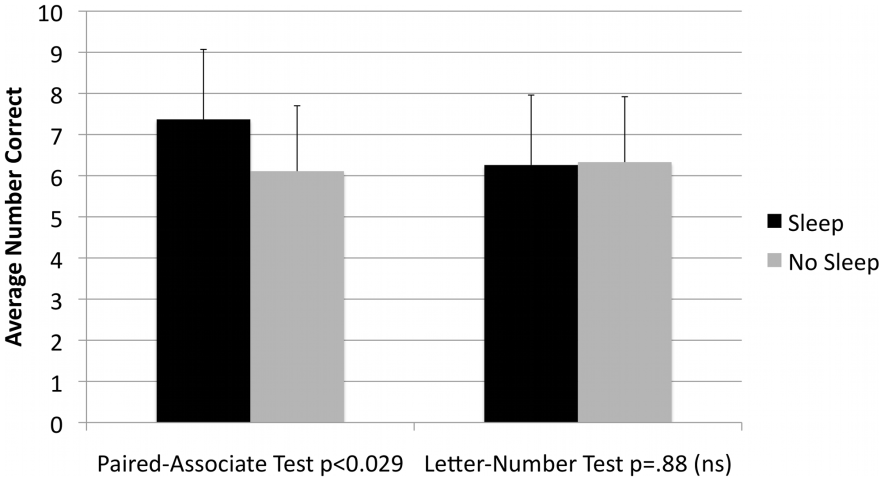
\includegraphics[width=\linewidth]{hypotheseGraph1}
		\caption{Conclusie studie Potkin en Bunney(2012)}
	\end{subfigure}
\end{figure}

Zoals je kan afleiden uit de boxplot uit week 1 omtrent slaap hoeveelheid verwachten we duidelijk dat mensen met een tekort aan slaap veel minder sterk zijn in het opnemen van nieuwe informatie. Maar in week 2 verwachten we eigenlijk dat het verschil iets minder groot zal zijn indien men iets minder slaap dan nodig heeft gehad, dit omdat men reeds het onderwerp heeft ingestudeerd op een voorgaand moment en men de kennis dus reeds heeft, men moet het enkel nog oproepen. Dit baseerden we op het artikel van \textcite{Potkin2012}.


\subsubsection{Hypothese omtrent muziek en Retrieval Practice}
\begin{figure}[H]
	\begin{subfigure}{0.45\textwidth}
		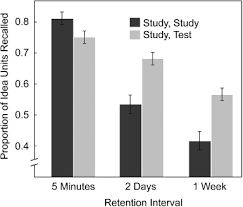
\includegraphics[width=0.8\linewidth]{hypotheseGraph2}
		\caption{Conclusie studie Roediger en Karpicke(2006)}
	\end{subfigure}
\end{figure}

In week 1 verwachten we dat mensen die niet naar muziek luisteren het aanzienlijk beter doen dan mensen die wel naar muziek luisteren, dit gestaafd door het artikel van \textcite{Dolegui2013}, het effect van retrieval practice in vergelijking met geen retrieval practice is hier nog niet zichtbaar.\\
\par
\noindent
In week 2 verwachten we dan weer meer een onderscheid tussen retrieval practice en geen retrieval practice, omdat men enkel kennis moet oproepen denken we dat muziek hier dus een kleiner effect heeft dan de invloed van retrieval practice. We denken dus dat retrieval practice hier zal uitblinken zoals je ook kan zien op de grafieken. Dit denken we vooral door het originele artikel van \textcite{Roediger2006}.
\section{Data}

Welke data hebben we nu juist onderzocht? Wel, zoals voordien vermeld hebben we eerst en vooral gekeken naar de verschillen tussen het niet gebruiken van “Retrieval Practice” en het wel gebruiken van deze methode, hierbij hebben we ook het effect van Muziek toegevoegd. Verder hebben we ook een apart onderzoek gedaan waarbij we opzoek gingen naar het effect dat de hoeveelheid slaap heeft op scores, losstaand van alle andere variabelen.\\
\par
\noindent
Eerst en vooral hebben we dus een script geschreven in R om het effect van slaap hoeveelheid te testen, hierbij hebben we drie verschillende ranges gedefinieerd: 0 tot 5 uur slaap, 5 tot 8 uur slaap en meer dan 8 uur slaap.\\
\par
\noindent
Verder hebben we ook boxplots gemaakt waarin we scores in 4 groepen onderverdeeld hebben, zo zien we een boxplot met scores waarbij men enkel naar muziek heeft geluisterd, een boxplot waarbij men naar muziek luisterde en Retrieval Practice heeft toegepast, een boxplot waarbij men enkel retrieval practice gebruikte en een boxplot met de overige scores
\section{Verklaringen}

\subsection{Slaap hoeveelheid}

Hierbij kwamen we tot de volgende grafieken voor week 1 en week 2:

\begin{figure}[H]
	\begin{subfigure}{0.45\textwidth}
		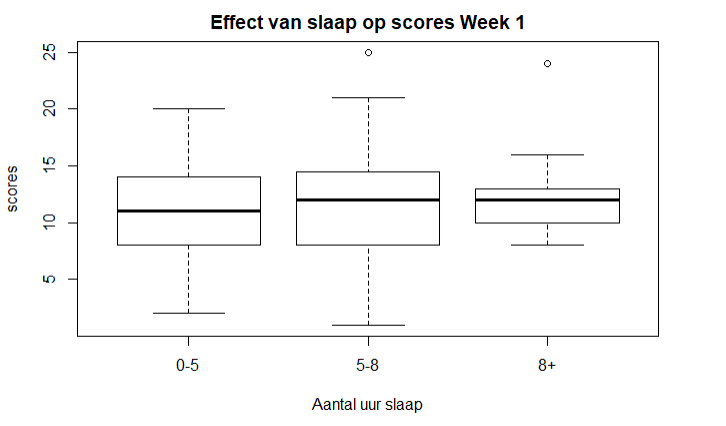
\includegraphics[width=\linewidth]{slaapGraph1}
	\end{subfigure}
\end{figure}

Hieruit kun je verschillende dingen afleiden, namelijk:

\subsubsection{Het effect van slaap op het instuderen van de leerstof. (Week 1)}

Hier kun je duidelijk zien dat slaap geen grote invloed heeft, maar er wel degelijk een invloed is, zo zie je dat het merendeel van de scores van mensen met minder dan 5 uur slaap toch iets lager liggen dan van mensen die voldoende slaap gehad hebben. Dit waarschijnlijk omdat het instuderen toch net iets moeilijker gaat als je weinig slaap hebt gehad

\subsubsection{Het effect van slaap op het behouden van ingestudeerde leerstof. (Week 2)}

Bij de tweede week is dit verschil nagenoeg volledig weggewerkt, voor het oproepen van kennis die men dus al heeft ingestudeerd maakt de hoeveelheid slaap dus eigenlijk niet echt uit.

\subsection{Retrieval Practice en Effect van Muziek}

Deze werden idem aan de voorgaande dataset ook geplot in R aan de hand van verschillende boxplots voor zowel week 1 als week 2

\subsubsection{De mate waarin je leerstof voor korte termijn kunt instuderen (Week 1)}

Eerst en vooral bekijken we welke invloed zowel Retrieval practice als Muziek hebben op het instuderen van leerstof.

\begin{itemize}
    \item Eerst en vooral hebben we het gebruik van muziek tegenover geen muziek.
    Hieruit kunnen we verrassend genoeg toch afleiden dat muziek een positief effect lijkt te hebben op het instuderen van de leerstof, aangezien de scores voor mensen die muziek gebruikt hebben om het gevraagde in te studeren een hogere score hebben, al dan niet met retrieval practice of niet, dan mensen die niet naar muziek geluisterd hebben.
    \item Hierna bekijken we het verschil tussen Retrieval Practice tegenover geen Retrieval Practice.
    Hier ziet men in de eerste testweek geen verschil tussen het al dan niet gebruiken van Retrieval Practice, tot dusver komt dit dus nog overeen met het originele artikel van Karpicke en Roediger waarop dit onderzoek gestaafd is.
    
\end{itemize}

\subsubsection{De mate waarin je kennis behoud op iets langere termijn (Week 2)}

Als laatste bestuderen we de grafiek voor de tweede week en kijken we bij welke methodes je kunt zien dat er toch een groter behoud aan kennis is.


\begin{itemize}
    \item Het gebruik van muziek tegenover geen muziek. Bij de tweede week is het “antwoord” toch niet meer zo eenduidig als het op muziek of geen muziek aankomt. Het verschil is aanzienlijk gezakt, wat toch blijk geeft dat indien men naar muziek luisterde in de eerste week men iets minder goed gememoriseerd heeft. Terwijl mensen die niet naar muziek luisteren wel net iets beter erin geslaagd zijn om hun kennis te behouden.
    
    Men ziet ook dat het al dan niet luisteren naar muziek niet echt een effect heeft op het oproepen van deze ingestudeerde kennis.
    
    \item Retrieval Practice tegenover geen Retrieval Practice. Hier is er ondertussen wel een duidelijk verschil zichtbaar, men ziet dat mensen die retrieval practice gebruikt hebben in de eerste week nu wel aanzienlijk beter scoren dan mensen die dit niet gedaan hebben, met uitzondering van mensen die geen retrieval practice hebben toegepast maar wel naar muziek hebben geluisterd, die even goed scoren als de groep die retrieval practice heeft gebruikt. 
    
    Hieruit kun je afleiden dat het al zeker beter is om retrieval practice toe te passen bij het instuderen, dan helemaal niets, wat overeenkomt met het originele artikel van Karpicke \& Roediger, maar dat het gebruik van enkel muziek (in dit geval erg rustige mozart) ook geen nefast effect heeft op het behouden van eerder verworven kennis.
    
\end{itemize}
    

\section{Resultaten \& Conclusie }

Het doel van deze studie was om te kijken of retrieval practice wel degelijk positieve invloed heeft op het onthouden van informatie (op lange termijn) en of muziek op zijn beurt nadelige effecten heeft erop. In totaal waren er 240 deelnemers in het onderzoek. Elke deelnemer moest een tekst van ongeveer een anderhalve A4 pagina lang lezen en hiervan zoveel mogelijk informatie onthouden. De deelnemers werden initieel in 2 groepen verdeeld: een groep die aan retrieval practice deed (en de methode STST toepast) en een groep die gewoon op het einde pas een test deed (SSST). Vervolgens werden deze 2 groepen verder verveeld in enerzijds een groep die naar muziek (klassiek) luistert en anderzijds een groep die niet naar muziek luistert. Tot slot houden we ook rekening met het aantal uur dat iemand geslapen heeft.

Als we kijken naar de resultaten van het onderzoek zien we dat Retrieval Practice het veel beter doet dan de gewone klassieke studiemethode. Echter de resultaten voor muziek en slaap zijn niet echt wat we verwacht hadden. Het verschil is gewoon te klein of het tegenovergestelde van wat we verwacht hadden en van de resultaten van <artikels>. We denken dat dit door de kwaliteit van het onderzoek komt. De tekst was vrij kort en ging over iets waar de meeste mensen al (veel) kennis over hadden, we denken dus dat het iets te makkelijk was, wat een verklaring is waarom de resultaten zo pover zijn. Ook zal het feit dat de deelnemers allemaal studenten waren voor dit vak, waarvan misschien een groot deel niet met alle positieve zin heeft deelgenomen, een invloed hebben. De verbetersleutel was volgens ons ook niet optimaal, er waren bijvoorbeeld 3 punten te verdienen met informatie over gemeenschappelijke voorouders (dit kon bijvoorbeeld samengenomen worden). Er was ook maar een week tussen de twee sessies, terwijl Retrieval Practice meer beloont als het over langere tijdsperioden gaat om informatie te onthouden.  Als laatste vinden we ook dat de verbetering hier niet optimaal gedaan is, aangezien dit door zoveel verschillende mensen gebeurd is, dit geeft verschillende perspectieven waardoor punten soms iets strenger of iets genereuzer bekomen konden worden. Kortom, we zijn sterk van mening dat het onderzoek veel beter kon en dat de resultaten hiervan zeker niet beslissend zijn en met een korrel zout moeten genomen worden, als je kijkt naar de resultaten van <onze artikels> waar (de invloed van) slaap en muziek beter bestudeerd werd.

%------------------------------------------------------------------------------
% Referentielijst
%------------------------------------------------------------------------------
% TODO: de gerefereerde werken moeten in BibTeX-bestand ``bibliografie.bib''
% voorkomen. Gebruik JabRef om je bibliografie bij te houden en vergeet niet
% om compatibiliteit met Biber/BibLaTeX aan te zetten (File > Switch to
% BibLaTeX mode)

\phantomsection
\printbibliography[heading=bibintoc]

\end{document}
